% This is "sig-alternate.tex" V2.1 April 2013
% This file should be compiled with V2.5 of "sig-alternate.cls" May 2012
%
% This example file demonstrates the use of the 'sig-alternate.cls'
% V2.5 LaTeX2e document class file. It is for those submitting
% articles to ACM Conference Proceedings WHO DO NOT WISH TO
% STRICTLY ADHERE TO THE SIGS (PUBS-BOARD-ENDORSED) STYLE.
% The 'sig-alternate.cls' file will produce a similar-looking,
% albeit, 'tighter' paper resulting in, invariably, fewer pages.
%
% ----------------------------------------------------------------------------------------------------------------
% This .tex file (and associated .cls V2.5) produces:
%       1) The Permission Statement
%       2) The Conference (location) Info information
%       3) The Copyright Line with ACM data
%       4) NO page numbers
%
% as against the acm_proc_article-sp.cls file which
% DOES NOT produce 1) thru' 3) above.
%
% Using 'sig-alternate.cls' you have control, however, from within
% the source .tex file, over both the CopyrightYear
% (defaulted to 200X) and the ACM Copyright Data
% (defaulted to X-XXXXX-XX-X/XX/XX).
% e.g.
% \CopyrightYear{2007} will cause 2007 to appear in the copyright line.
% \crdata{0-12345-67-8/90/12} will cause 0-12345-67-8/90/12 to appear in the copyright line.
%
% ---------------------------------------------------------------------------------------------------------------
% This .tex source is an example which *does* use
% the .bib file (from which the .bbl file % is produced).
% REMEMBER HOWEVER: After having produced the .bbl file,
% and prior to final submission, you *NEED* to 'insert'
% your .bbl file into your source .tex file so as to provide
% ONE 'self-contained' source file.
%
% ================= IF YOU HAVE QUESTIONS =======================
% Questions regarding the SIGS styles, SIGS policies and
% procedures, Conferences etc. should be sent to
% Adrienne Griscti (griscti@acm.org)
%
% Technical questions _only_ to
% Gerald Murray (murray@hq.acm.org)
% ===============================================================
%
% For tracking purposes - this is V2.0 - May 2012

\documentclass{sig-alternate-05-2015}

\usepackage{amssymb}
\usepackage[T1]{fontenc}
\usepackage{bbm}
\usepackage{amsthm}
\usepackage[utf8]{inputenc}
\usepackage{lipsum}
\usepackage{graphicx}
\usepackage[caption=false]{subfig}
\usepackage{graphicx}
\usepackage{csvsimple}
\usepackage{array}
\usepackage{float}
\usepackage{amsmath}
\usepackage{pgfplotstable}
\usepackage[demo]{graphicx}
\usepackage{subcaption}

\usepackage{amsmath}
\usepackage{algorithm}
\usepackage[noend]{algpseudocode}
\usepackage{varwidth}

\newtheorem{lemma}{Lemma}
\newtheorem{definition}{Definition}
\newtheorem{remark}{Remark}
\newtheorem{corollary}{Corollary}

\begin{document}
\nocite{*}
% Copyright
\setcopyright{acmcopyright}
%\setcopyright{acmlicensed}
%\setcopyright{rightsretained}
%\setcopyright{usgov}
%\setcopyright{usgovmixed}
%\setcopyright{cagov}
%\setcopyright{cagovmixed}


% DOI
\doi{10.475/123_4}

% ISBN
\isbn{123-4567-24-567/08/06}

%Conference
\conferenceinfo{PLDI '13}{June 16--19, 2013, Seattle, WA, USA}

\acmPrice{\$15.00}

%
% --- Author Metadata here ---
\conferenceinfo{WOODSTOCK}{'97 El Paso, Texas USA}
%\CopyrightYear{2007} % Allows default copyright year (20XX) to be over-ridden - IF NEED BE.
%\crdata{0-12345-67-8/90/01}  % Allows default copyright data (0-89791-88-6/97/05) to be over-ridden - IF NEED BE.
% --- End of Author Metadata ---
\title{Concept Drift Detection in Distributed Systems through LDA
Model Monitoring\titlenote{(Produces the permission block, and
copyright information). For use with
SIG-ALTERNATE.CLS. Supported by ACM.}}
\subtitle{[Extended Abstract]
\titlenote{A full version of this paper is available as
\textit{Author's Guide to Preparing ACM SIG Proceedings Using
\LaTeX$2_\epsilon$\ and BibTeX} at
\texttt{www.acm.org/eaddress.htm}}}
%
% You need the command \numberofauthors to handle the 'placement
% and alignment' of the authors beneath the title.
%
% For aesthetic reasons, we recommend 'three authors at a time'
% i.e. three 'name/affiliation blocks' be placed beneath the title.
%
% NOTE: You are NOT restricted in how many 'rows' of
% "name/affiliations" may appear. We just ask that you restrict
% the number of 'columns' to three.
%
% Because of the available 'opening page real-estate'
% we ask you to refrain from putting more than six authors
% (two rows with three columns) beneath the article title.
% More than six makes the first-page appear very cluttered indeed.
%
% Use the \alignauthor commands to handle the names
% and affiliations for an 'aesthetic maximum' of six authors.
% Add names, affiliations, addresses for
% the seventh etc. author(s) as the argument for the
% \additionalauthors command.
% These 'additional authors' will be output/set for you
% without further effort on your part as the last section in
% the body of your article BEFORE References or any Appendices.

\numberofauthors{8} %  in this sample file, there are a *total*
% of EIGHT authors. SIX appear on the 'first-page' (for formatting
% reasons) and the remaining two appear in the \additionalauthors section.
%
\author{
% You can go ahead and credit any number of authors here,
% e.g. one 'row of three' or two rows (consisting of one row of three
% and a second row of one, two or three).
%
% The command \alignauthor (no curly braces needed) should
% precede each author name, affiliation/snail-mail address and
% e-mail address. Additionally, tag each line of
% affiliation/address with \affaddr, and tag the
% e-mail address with \email.
%
% 1st. author
\alignauthor
Ran Bernstein\\
       \affaddr{Technion -- Israel Institute of Technology}\\
       \affaddr{Haifa 32000 Israel}\\
       \email{Bernstein.Ran@Gmail.com}
% 2nd. author
\alignauthor
 Daniel Keren\\
       \affaddr{Haifa University}\\
       \affaddr{Haifa 31905 Israel}\\
       \email{dkeren@cs.haifa.ac.il}
% 3rd. author
\alignauthor 
Margarita Osadchy\\
       \affaddr{Haifa University}\\
       \affaddr{Haifa 31905 Israel}\\
       \email{rita@cs.haifa.ac.il }
\and  % use '\and' if you need 'another row' of author names
% 4th. author
\alignauthor Assaf Schuster\\
       \affaddr{Technion -- Israel Institute of Technology}\\
       \affaddr{Haifa 32000 Israel}\\
       \email{assaf@cs.technion.ac.il}
}
% There's nothing stopping you putting the seventh, eighth, etc.
% author on the opening page (as the 'third row') but we ask,
% for aesthetic reasons that you place these 'additional authors'
% in the \additional authors block, viz.
\additionalauthors{Additional authors: John Smith (The Th{\o}rv{\"a}ld Group,
email: {\texttt{jsmith@affiliation.org}}) and Julius P.~Kumquat
(The Kumquat Consortium, email: {\texttt{jpkumquat@consortium.net}}).}
\date{30 July 1999}
% Just remember to make sure that the TOTAL number of authors
% is the number that will appear on the first page PLUS the
% number that will appear in the \additionalauthors section.

\maketitle
\begin{abstract}
Real systems for mining dynamic data streams should be able to detect changes that affect the 
accuracy of the global model. The majority of previous work addressed the centralized settings 
and proposed solutions, based on the statistics of error rates in the data stream.
In this work, we focus on distributed settings. 
Model training in a distributed environment 
requires centralizing the data from all nodes (synchronization), which is very
costly in term of communication.
In order to minimize the communication, a monitoring algorithm should be done locally at each node, 
while preserving the validity of the global model. 
We propose a first communication-efficient algorithm for monitoring a classification model over 
distributed, dynamic data streams. Linear Discriminant Analysis (LDA) is a popular algorithm 
used for classification and dimensionality reduction in many fields, thus we use LDA as our 
classification model. 
Our algorithm has strong theoretical guarantees of correctness and it is shown empirically to 
reduce communication volume by up to two orders of magnitude on three completely different 
real data sets. Moreover, our approach monitors the classification model itself as opposed 
to its errors, which allows to detect the change before the error occurs.
\end{abstract}


%
% The code below should be generated by the tool at
% http://dl.acm.org/ccs.cfm
% Please copy and paste the code instead of the example below. 
%
\begin{CCSXML}
<ccs2012>
 <concept>
  <concept_id>10010520.10010553.10010562</concept_id>
  <concept_desc>Computer systems organization~Embedded systems</concept_desc>
  <concept_significance>500</concept_significance>
 </concept>
 <concept>
  <concept_id>10010520.10010575.10010755</concept_id>
  <concept_desc>Computer systems organization~Redundancy</concept_desc>
  <concept_significance>300</concept_significance>
 </concept>
 <concept>
  <concept_id>10010520.10010553.10010554</concept_id>
  <concept_desc>Computer systems organization~Robotics</concept_desc>
  <concept_significance>100</concept_significance>
 </concept>
 <concept>
  <concept_id>10003033.10003083.10003095</concept_id>
  <concept_desc>Networks~Network reliability</concept_desc>
  <concept_significance>100</concept_significance>
 </concept>
</ccs2012>  
\end{CCSXML}

\ccsdesc[500]{Computer systems organization~Embedded systems}
\ccsdesc[300]{Computer systems organization~Redundancy}
\ccsdesc{Computer systems organization~Robotics}
\ccsdesc[100]{Networks~Network reliability}


%
% End generated code
%

%
%  Use this command to print the description
%
\printccsdesc

% We no longer use \terms command
%\terms{Theory}

\keywords{ACM proceedings; \LaTeX; text tagging}

\section{Introduction}
In this work, we address the problem of mining data streams when the streaming data is 
{\em distributed} over a large number of nodes. We assume that the data generation 
process and the prediction problem is the same for all nodes. An important challenge, 
associated  with real life problems, is that the distribution of the streaming 
data is not stationary, notably, it can change over time. 
The change could be caused by a system fault (e.g. sensor failure) or by a transition 
in the target concept. 
Classical examples of a prediction problem that involves target 
concept change are user preference prediction and fraud detection. 
In the former, the choices of the user can change over time; in the latter, the fraudulent 
transactions change constantly to avoid detection. 
In both, the target concept changes over time, and if not detected, renders the prediction model inadequate.

Methods that detect changes in data over time are referred to as {\em concept drift detection} or {\em change-point detection}. 
A large volume of work has been done on these topics 
(see e.g.~\cite{basseville1993detection,brodsky2013nonparametric,ChenGupta2000,Tsymbal,Gama2014} 
for in-depth survey of the field).
The solutions, proposed in previous work, cover different forms of change in the data, i.e. 
the input data characteristics, or the relation between the input data and the target variable, or both. 
Some forms of change will influence the prediction model and some will not  
(even though these changes could be detected as a distribution switch). 
In this work, we are only concerned with the changes that affect the model.
Our method is distinct from the previous work in the following important aspects:
\begin{description}
\item[Model-Based Monitoring] In this work, we focus on monitoring a classification model. 
Most previous work on concept drift detection~\cite{baena2006early,gama2004learning,Nishida2007}, 
concerned with classification, are error-based  (they utilize classification error rates to 
draw conclusion about the change of the distribution). 
Here, we propose to monitor the change in the {\em model} itself as opposed to errors in classification.  
Monitoring the model and not the errors has an important benefit, which is detecting the 
drift before  the prediction error occurs.

\item[Distributed Setting]
    Concept drift has been actively studied in centralized settings. 
    We are one of the very few works \cite{AngGZPH13} that detects concept drift in a distributed 
    environment, which is a critical part of a real big data system.
    In such systems, data is distributed over a large number of nodes and the model is learned 
    in a global way, after the data is centralized from all nodes (hereafter, synchronization). 
    This process requires a lot of resources and communication. 
    Thus it is crucial to minimize the number of synchronisations. 
    Our approach for monitoring the global model over a distributed system  
    provides provable guarantees of correctness, while existing methods for detection of concept 
    drift in distributed settings~\cite{AngGZPH13} rely on heuristics, utilizing error rate statistics.
\end{description}


Similarly to~\cite{icml2014c2_harel14}, we link the concept drift detection method with the 
hypothesis class and the training algorithm  
In this paper we focus on linear binary classifiers as a hypothesis class, and
Linear Fisher Discriminant \cite{fisher1936use} as the learning algorithm. We focus on linear classifiers, as they are well studied, allowing a solid platform for analysing new concepts. Linear classifiers are also very popular in real applications and serve as a platform for more complex classifiers, such as ensemble models~\cite{Deva, eSVM},
neural networks~\cite{osadchy2015k}, and even deep architectures\cite{ROSS}.


\subsection{Our Contribution}
We propose Distributed Linear Discriminant Analysis (DLDA): a novel
communication-efficient algorithm for monitoring LDA classifier over a distributed, dynamic data streams.
The proposed approach monitors the {\em model} itself, rather than classification errors 
and detects concept drift in streaming data, before the errors occur. 
The algorithm is designed for {\em distributed setting}, and it has strong 
{\em theoretical guarantees} of correctness. 
We show empirically on three completely different real data sets that the proposed 
method reduces communication volume by up to two orders of magnitude.


\section{Related Work}
\subsection{Distributed Monitoring}
In the last few years there has been an increase in work on defining local tests 
for monitoring a function that depends on data distributed over nodes.
Most of the work so far has been with simpler functions such as linear
\cite{keralapura2006communication, kashyap2008efficient} and monotonic \cite{michel2005klee}.
For non-linear functions, examples include work on monitoring
the value of a single-variable polynomial \cite{shah2008handling}, 
and eigenvalue perturbation \cite{huang2007communication}. 
A generic geometric approach for monitoring arbitrary functions is proposed in
\cite{sharfman2007geometric}, and later extended and generalized
\cite{keren2012shape,lazerson2015monitoring}. 
The closest work to ours is on Least Square Regression
\cite{gabel2015monitoring}. We build upon some of the results from
\cite{gabel2015monitoring}, but the problem definition in LDA monitoring is much
more complex.
%and we will harness some of their mathematical lemmas for our LDA problem. 

A great part of the difficulty in monitoring the LDA formula derives from the
need to monitor matrix inversion, which is not linear or convex,
and the number of monomials explodes exponentially when written explicitly
(what makes it infeasible to apply one of the polynomial tracking
algorithms).
\subsection{Concept Drift Detection}

Popular approaches for detecting concept drift identify the change point
\cite{gama2004learning,wang2013concept}. Drift Detection Method (DDM) is the
most widely used concept drift detection algorithm designed strictly for streaming data 
\cite{gama2004learning}. DDM use the sum of overall classification error and 
its empirical standard deviation and hence fails to detect a drift unless the
error rate changes, without considering where the error occur.
The Early Drift Detection Method (EDDM) \cite{baena2006early} achieves better
detection results than DDM if the data stream has changes gradually.
EDDM monitors the distance between the two classification errors. 
Linear Four Rates (LFR) \cite{wang2015concept} uses as a statistic a linear
combination of all history errors, with a decay parameter. The approach 
specified in \cite{klinkenberg2000detecting,dries2009adaptive} makes use of
the SVM error for detection. DDM, EDDM, LFR and SVM related approaches focus
their analysis on the error and not on the model itself, and do not supply a
theoretical guarantee on the validity of the global (of distributed setting) 
model of a specific classification algorithm (such as LDA in our case).
\subsection{Linear Discriminant Analysis}%\\ \par
LDA seeks for a linear combination of features that
characterize or separate two or more classes of objects or events.
The resulting combination may be used as a linear classifier, or,
more commonly, for dimensionality reduction before later classification.

In LDA the problem is approached by assuming that the conditional probability
density functions $P(\vec x|y=p)$ and $P(\vec x|y=q)$ are both normally distributed with
mean and covariance parameters $\left(\vec \mu_p, B_p\right)$ and
$\left(\vec \mu_q, B_q\right)$, for two target classes p and q respectively.
${(x_1,y_1),\ldots,(x_n,y_n)}$ are I.I.D samples, $x_i \in \mathbb{R}^d$
and $y_i \in \{0,1\}$.

% Let ${(x_1,y_1),\ldots,(x_n,y_n)}$ be a set of n observation pairs of $d < n$
% independent variables and one dependent variable, where $x_i$ are column vectors in $\mathbb{R}^d$, and $y_i$ are the
% corresponding classes.
We seek a linear transformation (model), $w \in \mathbb{R}^d $,
that maximizes the separation between the classes, where the separation is
defined to be the ratio of the variance between the classes to the variance
within the classes:
\begin{equation*}
S := \frac{\sigma^2_{between}}{\sigma^2_{within}} = \frac{(w \dot (\mu_p -
\mu_q))^2}{w^T(B_p+B_q)w}.
\end{equation*}
Under this assumption, the Bayes optimal decision criterion is a threshold on the
dot product
\begin{equation*} \label{eq:decision}
w \cdot x > c
\end{equation*}
for some threshold constant c, where
\begin{equation} \label{eq:w}
w \propto (B_p+B_q)^{-1}(\mu_p - \mu_q)
\end{equation}
\begin{equation} \label{eq:c}
c = \frac{1}{2}(T-{\mu_p}^T S_p^{-1} {\mu_p}+{\mu_q}^T S_q^{-1} {\mu_q}).
\end{equation}
In this work we monitor $w$, and will refer it as the
classifier's \textit{model}.
 
\section{Theoretical Foundation}
\subsection{Problem Definition}
We denote $k$ as the number of nodes.
$n$ is the number of vectors in a node.
$x^i_j$ and $y^i_j$ are the j'th vector and label in the i'th node.
Assume that the observations ${(x^i_j; y^i_j)}$ are distributed across k nodes, 
and that these observations are dynamic (they change over time, as nodes receive 
new observations that replace older ones). 
As data evolves, it is possible that the previously computed model no longer 
matches the current true model. 
Let $w_0$ be the existing model (vector of weights of a linear classifier), 
previously computed at some point in the past (the synchronization time), 
and let $w$ be the true (if we had aggregated the current observations 
from all of the nodes into one place and computed the model according to it) LDA
model.
We wish to maintain an accurate estimation $w_0$ of the current global LDA model, $w$. 
The question is then when to update the model.
Given an error threshold $T$, our goal is to raise an alert if
\begin{equation} \label{eq:coneCritiria}
\frac{<w,w_0>}{\parallel w \parallel \parallel w_0 \parallel}  < T.
\end{equation}
Due to the complexity of Eq. \ref{eq:coneCritiria},
we will monitor a simpler problem that its solution also satisfies
Eq. \ref{eq:coneCritiria}: the maximal volume sphere that $w_0$ is its center
that resides completely inside the cone from Eq. ~\ref{eq:coneCritiria}.
This sphere is defined by
\begin{equation} \label{eq:critiria}
\parallel w-w_0 \parallel \  >  R_0,
\end{equation}
where $R_0 := \  \parallel w_0 \parallel \sqrt{1-T^2}$ is its radius.
When $w_0$ and $w$ norms do not change significantly \ref{eq:coneCritiria} and
\ref{eq:critiria} match (a small angle between unit vectors is
equivalent to a small norm of the subtraction between them).
Empirical testing of the difference between Eq. \ref{eq:coneCritiria} and
Eq. \ref{eq:critiria} has showed that they are almost interchangeable for the
purpose of concept drift detection, i.e., when data changes there is a high
correlation between the values of $1-\frac{<w,w_0>}{\parallel w \parallel
\parallel w_0 \parallel}$ and $\parallel w-w_0 \parallel $.

\subsection{Monitoring Distributed LDA With Convex Subsets}
Monitoring distributed LDA models is difficult because the
global model cannot be inferred from the local model at each
node. Even when all current local models $w_i$ are similar to the precomputed
local models $w_0$, the current global model $w$ may
be very different from the precomputed model $w_0$. Consider
the example in Figure \ref{NegativeExampl} with $k = 2$ nodes and dimension $d =
2$. The global model's angle deviation is large (45 degrees) even
though the local models are identical to what they were at the initial
point.

\begin{figure}[h]
\centering
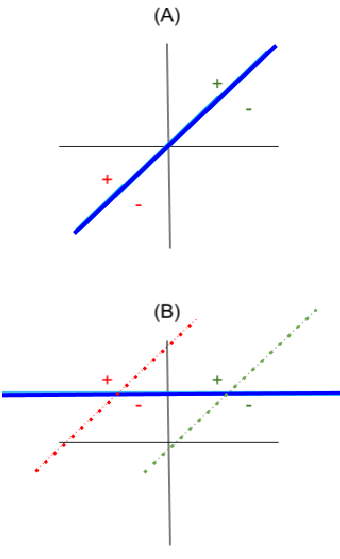
\includegraphics[width=60mm]{NegativeExample.png}
\caption{Example of false monitoring by applying the LDA formula locally. The
initial state of the data is presented in (A) and the state at a later point
is shown in (B). In (B) every node (green and red) calculates the same angle
for the separator as it was in (A). But it can be
seen that the true separator's (blue dashed line) angle has changed
significantly. (Best to use in color)}
\label{NegativeExampl}
\end{figure}


\\\par To overcome this difficulty, we turn to geometric monitoring. Geometric
monitoring \cite{keren2014geometric, keren2012shape} is a communication
efficient approach that monitors whether a function of distributed
data streams crosses a threshold. The key idea is to
impose constraints on local data at the nodes, rather than
on the function of the global aggregate. Given a function of
the average of all local data and the threshold, we compute a
``good'' convex subsets, called \textit{safe zones}, for each
node.
\\\par As we show below, convexity
plays a key role in the correctness of this scheme. As long
as local data stay inside the safe zones, we guarantee that
the function of the global average does not cross a threshold (that is given
in terms of maximal angle or norm of distance between the classifiers).
Nodes communicate only when local data drifts outside the
safe zone, which we call a safe zone \textit{violation} ((hereafter,
violation)). Once that happens, violations can be resolved, for example by gathering
data from all nodes and recomputing $w_0$ and the safe zones.
In other words, we want to impose conditions on the local
data at each node so that as long as they hold, $||w-w_0||<R_0$.

\subsection{Notation}
$p,q,p^i$ and $q^i$  are the global and local mean of the classes.
\\$S$ and $S^i$  are the global and local normalized scatter matrices:
\\$S^i := \frac{1}{n}\sum_{j=1}^{n}x^i_j(x^i_j)^T
\\S := \frac{1}{nk}
\sum_{i=1}^k\sum_{j=1}^nx^i_j(x^i_j)^T=\frac{1}{k}\sum_{i=1}^kS^i$.
\\Similarly, $u$ and $u^i$ are the distance between the classes means
\\$u:=p - q$
\\$u^i:=p^i - qi$.
\\ $B$ is the global covariance matrix which is the sum of the covariance
matrices of the two classes:
\\$B:=B_p+Bq$
\\$B=S - pp^T - qq^T$.
%\\B^i:=S^i - p^i(p^i)^T - q^i(q^i)^T$
\\\\Let w be our current true model. Then, following Eq.~\ref{eq:w}, we can
denote:
%\\$w(S,\mu_p,\mu_q) := (S - \mu_p\mu_p^T - \mu_q\mu_q^T)^{-1}(\mu_p - \mu_q)$
\begin{equation*}
w:=(S - pp^T - qq^T)^{-1}(p-q)=B^{-1}u.
\end{equation*}
Let $w_0$ be the existing model, previously computed from $(S_0, p_0, q_0)$
or from $(B_0,u_0)$ at some point in the past (the synchronization time).
Then,
\begin{equation*} 
w_0:=(S_0 - p_0p_0^T - q_0q_0^T)^{-1}(p_0-q_0)=B_0^{-1}u_0.
\end{equation*}
$\Delta_s, \delta_p$, and $\delta_q$ are the drift vectors of $S, p$, and $q$,
i.e.,
\begin{alignat*}{1}
& \Delta_s:= S - S_0 \\
& \delta_p:= p - p_0 \\
& \delta_q := q - q_0.
\end{alignat*}
\\If $S_0^i$, $p_0^i$ and $q_0^i$ are the local normalized scatter and averages
of the samples in a node, we can define the local drifts to be:
\begin{alignat*}{1}
& \Delta_s^i:= S^i - S_0^i
\\ & \delta_p^i:= p^i - p_0^i
\\ & \delta_q^i:= q^i - q_0^i.
\end{alignat*}
\begin{remark} \label{average}
It is easy to see that every global drift is the average of the local drifts:
\begin{alignat*}{1}
& \Delta_s = \frac{1}{k} \sum \Delta_s^i, \\
& \delta_p = \frac{1}{k} \sum \delta_p^i, \\
& \delta_q = \frac{1}{k} \sum \delta_q^i.
\end{alignat*}

\end{remark}

\subsection{Convex Safe Zones}
Each node monitors its own drift: as long as current values
at local nodes $(S^i,p^i,q^i)$ are sufficiently similar to their values
at synchronization time $(S^i_0,p^i_0,q^i_0)$, $w_0$ is guaranteed to be close to $w$.
Formally, we define a convex subset $\mathcal{C}$ such that:
\begin{equation} \label{convex}
(\Delta_s, \delta_p, \delta_q) \in \mathcal{C} \Rightarrow \parallel w-w_0
\parallel \ < R_0.
\end{equation}
\begin{lemma}
Let $\mathcal{C}$ be a convex subset that satisfies Eq. \ref{convex}.
If $(\Delta_s^i, \delta_p^i, \delta_q^i) \in \mathcal{C}$ for all i, then
\begin{equation*}
\parallel w-w_0 \parallel \ < R_0.
\end{equation*}
\end{lemma}
\begin{proof}
Express $S, p$ and $q$ as their values at synchronization with the addition of the
average of the local drifts:
\begin{equation*} 
\begin{split}
(S,p,q) & = \frac{1}{k} \sum_i (S^i,p^i,q^j) \\
 & = (S_0,p_0,q_0) + \frac{1}{k} \sum_i (\Delta_s^i,\delta^i_p,\delta_q^i). \\
\end{split}
\end{equation*}
From $\mathcal{C}$'s convexity and using Remark \ref{average} we get:
\begin{equation*} 
\begin{split}
\forall i (\Delta_s^i,\delta^i_p,\delta_q^i) \in \mathcal{C} & \Rightarrow 
\frac{1}{k} \sum_i (\Delta_s^i,\delta^i_p,\delta_q^i) \in \mathcal{C} \\
& \Rightarrow (\Delta_s,\delta_p,\delta_q) \in \mathcal{C}.
\end{split}
\end{equation*}
Finally, from the definition of $\mathcal{C}$ we obtain:
\begin{equation*}
(\Delta_s,\delta_p,\delta_q) \in \mathcal{C} \Rightarrow \parallel w-w_0
\parallel \ < R_0,
\end{equation*}
which completes the proof.
\end{proof}

\subsection{Sliding Window Convex Bound}
In the sliding window model each node computes $S^i$ from the $L$ samples seen
at node $i$, while $S_0^i$ (and hence $S_0$) is built from the last L samples before
synchronization. 
We denote the drift in the global covariance matrix
\begin{alignat*}{2}
\Delta & := && B-B_0 \\
& = && (S_0+\Delta_S - (p_0+\delta_p)(p_0+\delta_p)^T \\
& && - (q_0+\delta_q)(q_0+\delta_q)^T) \\
& && - (S_0 - p_0p_0^T - q_0q_0^T) \\
& = && - \delta_p\delta_p^T - \delta_q\delta_q^T \\
& && + \Delta_S - p_0\delta_p^T \\
& && - \delta_pp_0^T - q_0\delta_q^T - \delta_qq_0^T.
\end{alignat*}
We break $\Delta$ into its quadratic part,
\begin{equation*}
M:= - \delta_p\delta_p^T - \delta_q\delta_q^T,
M^i:= - \delta_p^i(\delta_p^i)^T - \delta_q^i(\delta_q^i)^T, 
\end{equation*}
and its linear part,
\begin{equation*}
L:= \Delta_S - p_0\delta_p^T - \delta_pp_0^T - q_0\delta_q^T - \delta_qq_0^T, 
L^i := \Delta_S^i - p_0^i(\delta_p^i)^T - \delta_p^i(p_0^i)^T -
q_0^i(\delta_q^i)^T - \delta_q^i(q_0^i)^T,
\end{equation*}
and hence 
\begin{equation*}
\Delta= L+ M.
\end{equation*}
We denote the drift of the distance between the means:
\begin{equation*}
\delta:= u-u_0 = \delta_p - \delta_q.
\end{equation*}
Now we can state a convex bound for our problem:
\begin{lemma} \label{convexBound}
If $\mathcal{G}$ is the set of triplets $(\Delta_s^i, \delta_p^i, \delta_q^i)$
 that satisfies the bound:
 \begin{equation} \label{eq:convexBound}
\begin{split}
||B_0^{-1}\delta|| &+ (||w_0||+R_0)(||B_0^{-1}L||+||B_0^{-1}M||) \\ & \leq  R_0
\end{split}
\end{equation}
and satisfies the inequality:
 \begin{equation*} 
||B_0^{-1}\Delta|| < 1
\end{equation*}
 then $\mathcal{G}
 \subseteq \mathcal{C}$ and $\mathcal{G}$ is convex, where $||A||$ is the
 operator norm of the matrix A.
\end{lemma}
The proof of lemma \ref{convexBound} is given in Appendix A.

\section{Method}
In this section we will present two frameworks for LDA model monitoring that use
bound \ref{eq:convexBound}. In both of the frameworks, every node runs the same
update algorithm as detailed in Alg. \ref{NodeUpdate}. 
The frameworks differ in their violation recovery policy. 
The first --- Distributed LDA Monitoring (DLDA) -- will synchronize in a round
that at least one node has reported a violation in it as it detailed in Alg.
\ref{DLDA}.
The second --- Probabilistic Distributed LDA Monitoring (PDLDA) -- will synchronize in
a round that the number of violations in it is above a certain threshold.
The calculation of this threshold is presented in the subsection below.


\begin{algorithm}
\caption{Node i update with new samples x; y.
\\$x_{old}^i(p)$ and $x_{old}^i(q)$ are the oldest samples from each class in the
sliding window of the i'th node.}\label{NodeUpdate}
\begin{algorithmic}[1]
\Procedure{Update}{}
\If {$y$ is class P} 
\State $p^i = p^i + x - x_{old}^i(p)$
\State $S^i = S^i +xx^T - x_{old}^i(p)*(x_{old}^i(p))^T$
\Else 
\State $q^i = q^i + x -x_{old}^i(q)$
\State $S^i = S^i +xx^T - x_{old}^i(q)*(x_{old}^i(q))^T$
\EndIf
\State $(\Delta_s^i,\delta^i_p,\delta_q^i) = (S^i-S^i_0,p^i-p^i_0,q^i-q^i_0)$
%\If{The bound in \ref{eq:convexBound} is not satisfied}

\If { \begin{varwidth}[t]{\linewidth}
$||B_0^{-1}\delta^i||+ (||w_0||+R_0)(||B_0^{-1}L^i||+||B_0^{-1}M^i||) $ \par
\hskip\algorithmicindent $>R_0$} 
\end{varwidth}
\State Report violation to coordinator
\State Receive new global $B_0^{-1}$, $||w_0||$
\State $(S_0^i,p_0^i,q_0^i) = (S^i,p^i,q^i)$
\EndIf

\EndProcedure
\end{algorithmic}
\end{algorithm}

\begin{algorithm}
\caption{Coordinator violation resolution algorithm.}\label{DLDA}
\begin{algorithmic}[1]
\Procedure{Sync}{}
\If {One of the nodes has reported for violation} 
\State Receive from every node $i$ the triplet $(S^i,p^i,q^i)$
\State Compute updated $||w_0||$ and $B_0^{-1}$ and distribute.
\EndIf
\EndProcedure
\end{algorithmic}
\end{algorithm}

\subsection{Probabilistic Distributed LDA Monitoring}
As it will be seen in the evaluation section, DLDA is too strict when handeling
a big number of nodes: practically, syncing every time that a single node
has a violation causes a lot of redundant synchronizations, i.e., every node i
sends $(S^i,p^i,q^i)$ even though the global model is valid (close enough
to the model that was computed at last synchronization). The redundant
synchronization increase communication unnecicerily due to the limited ability 
of the convex bound that is tested localy to reflect the true global error.
To solve this problem, we would like to enjoy from the fact that we deal with 
big number of nodes: we propose in this section a
probabilistic framework for applying the bound in a way that reduces the number of redundant syncs (Others might consider
to embed our bound in a different framework). 
We call ours Probabilistic Distributed LDA Monitoring (PDLDA) and its
empiric evaluation validate our assumption for reducing the redundant syncs.
The basic idea is not to synchronize when a single node is violated but only 
when the number of violations is above a certain threshold. 
This approach is based on the assumption that in an stationary system, 
the probability for a local violation in a node remains approximately the same
when the true (global) error rate stays low. 
Let $U \in {0,1}$ be an indicator of an increase in the true model error,
and let $v_i \in {0,1}$ be an indicator for a local violation in the
i'th node. We define the probability for True Positive (TP) and False Positive
(FP) in a node as:
\begin{alignat*}{1}
& P_{TP} := P(v_i=1 | U=1) \\
& P_{FP} := P(v_i=1 | U=0).
\end{alignat*}
Let $V$ be the random variable denoting the number of local violations
\begin{equation*}
V := \sum_{i=1}^k v_i.
\end{equation*}
We would like to derive a condition that for a given $0 < \epsilon < 0.5$
indicates an increase of the true error (the norm of
the distance between the current model to the last one that was computed) 
with high probability in the following form:
$P(V=v|U=0) < \epsilon$.
\\We denote the minimal number of violations that cause a synchronization as a violation
threshold $t$ and it is quantified by $t:=k*P_{FP}+z$ for some integer $z$.
From the Chernoff bound it follows that 
\begin{alignat*}{1}
& P(V>t) \\
& = P(V>k*P_{FP}+z) \\
& \leq \exp(-\frac{z^2}{2kP_{FP}(1-P_{FP})}) \\
& \leq \epsilon.
\end{alignat*}
For $z^*:=\sqrt{2kP_{FP}(P_{FP}-1)\log(\epsilon)}$ the condition is satisfied. 
We denote $t^*:=k*P_{FP}+z^*$; therefore we get $P(V > t^*) <
\epsilon$ when the true error is steady.
We can state this simply by saying that, with high probability, $V > t^*$
indicates an increase in the global error and that becomes our rule for a
sync.
\section{Evaluation}
We evaluated the performance of our monitoring algorithms,
DLDA and PDLDA, using simulations with synthetic and real-world 
distributed datasets. 
For each dataset we simulated the nodes and the coordinator, 
counted synchronization s, and kept track of the resulting true models $w$ and the
current monitored models $w_0$. 
\subsection{Synthetic Data Experiments}
We compared DLDA to the T-periodic algorithm, denoted
PER(P), a simple sampling algorithm that sends updates
every P rounds. Though PER cannot guarantee a bound for the
error, it can achieve arbitrarily low communication.
Our main performance metric is communication, measured
in \textbf{normalized messages} --- the average number of messages sent per
round by each node. Note that DLDA \textit{guarantees}
a global error below a given $T$ while PER does not.

\begin{figure*}[ht]
	\centering
	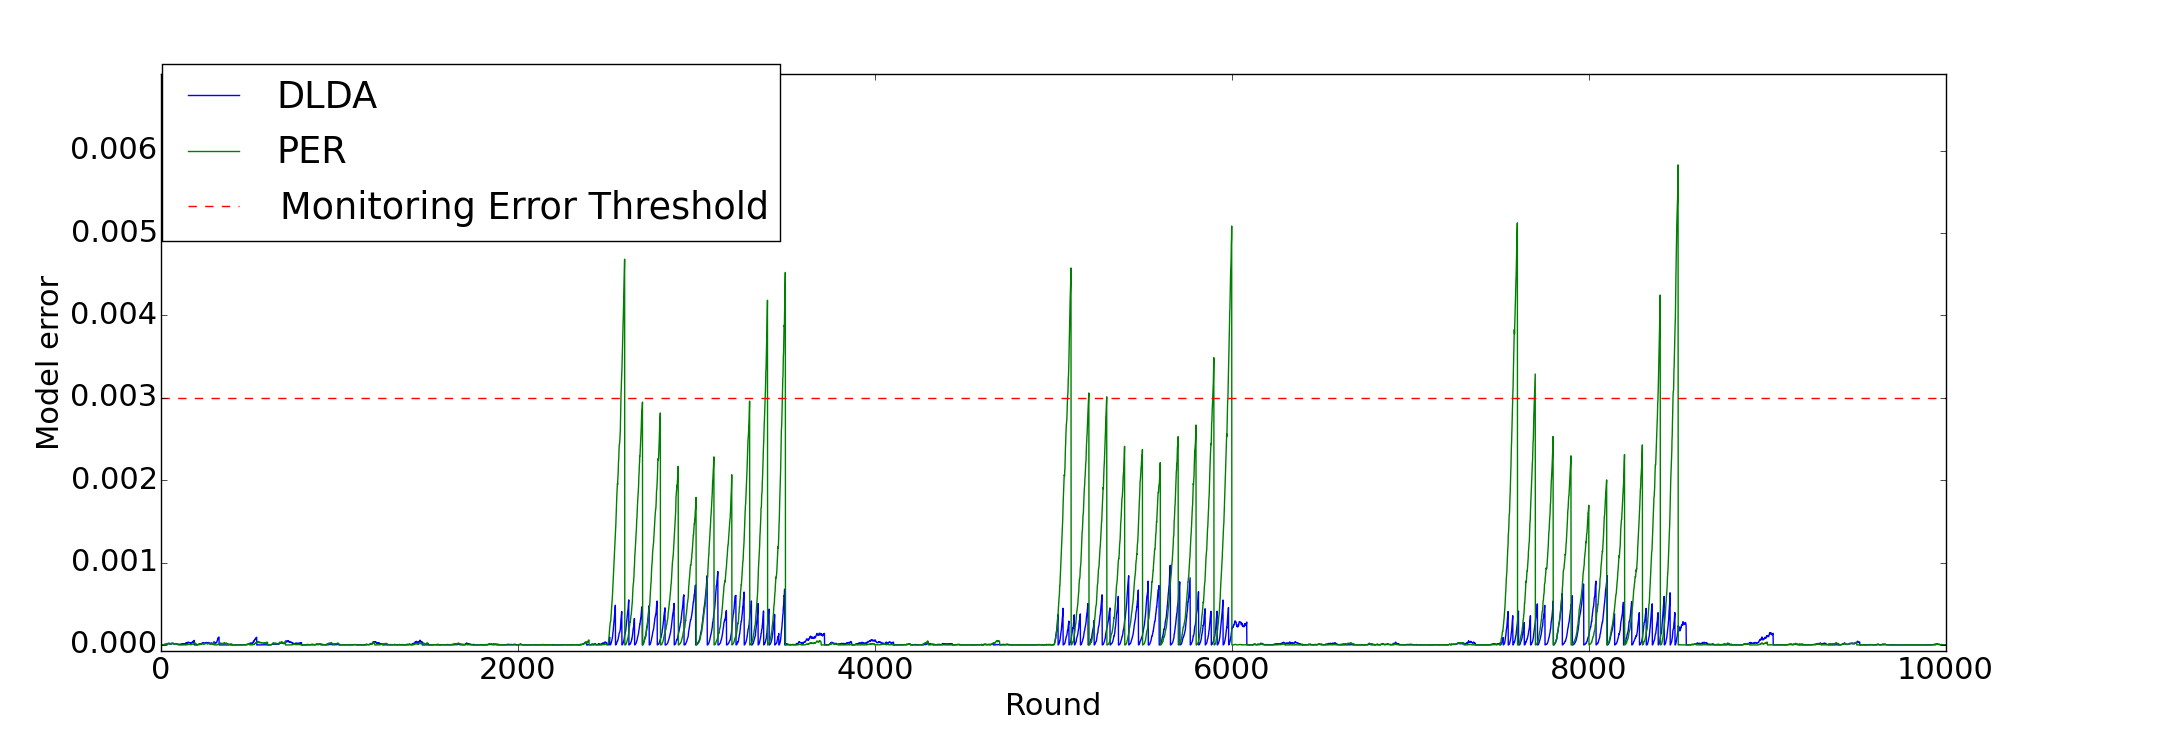
\includegraphics[width=\textwidth]{PER/PERvsDLDAoverTime.png}
	\caption{ DLDA model error (blue) compared to PER(100) model error (green), 
	for k = 10 simulated nodes with d = 2 dimensions, threshold T = 0.99 and
	window size L=1000. Both algorithms reduce communication to 1\%, but DLDA
	only synchronizes when $w$ changes. PER(100) synchronizes every 100 rounds, 
	but is unable to maintain error below the threshold (dashed horizontal line).}
	\label{PERvsDLDAoverTime}
\end{figure*}
	
Figure \ref{PERvsDLDAoverTime} shows the behavior of the monitoring 
algorithm over a simulation on a dataset with 3 concept drifts. 
DLDA achieves communication of 0.01 messages per node per round, and 
the model error is always below the threshold. 
Conversely, the equivalent PER(100) algorithm doesn't maintain the
error below the threshold. 
It can be seen that the periodic algorithm 
not only has an error rate above the required threshold but also
synchronizes between the concept drifts when there is no reason to do so.
\subsubsection{Threshold}
Figure \ref{PERvsDLDAoverError} shows the communication required for different
threshold levels for the DLDA algorithm, and the minimal
communication required to match DLDA using the PER.	
It can been seen that for both fixed and drift data, DLDA outperforms PER for
any given error threshold.
 \begin{figure}[ht]
	\centering
	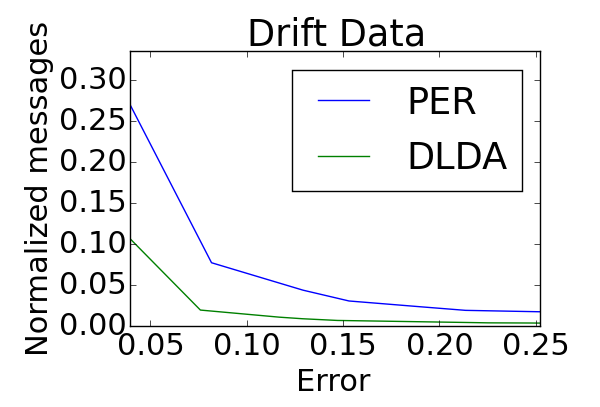
\includegraphics[width=60mm]{PER/onlyDrift.png}
	\caption{Communication for DLDA (blue) and the
	periodic algorithm tuned to achieve the same max error
	(green) at different threshold values.}
	\label{PERvsDLDAoverError}
	\end{figure}

	
\subsubsection{Node Scalability}
Figure \ref{Nodes} shows communication for different numbers of nodes k. 
We observe that communication increases slowly, reaching to 0.25\% for fixed
data and 0.6\% for drift data for 25 nodes.
	\begin{figure}[h]
	\centering
	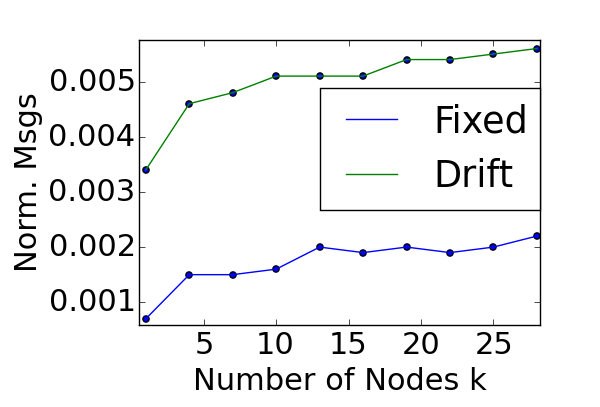
\includegraphics[width=60mm]{CommunicationOfFixedVsDrift/Nodes.png}
	\caption{Communication as a function of the number of nodes}
	\label{Nodes}
	\end{figure}
\subsubsection{Dimension}
Figure \ref{Dimension} shows how the dimension of the dataset affects
communication.
When window size $W$ is fixed, communication grows linearly with dimension $d$.
	\begin{figure}[h]
	\centering
	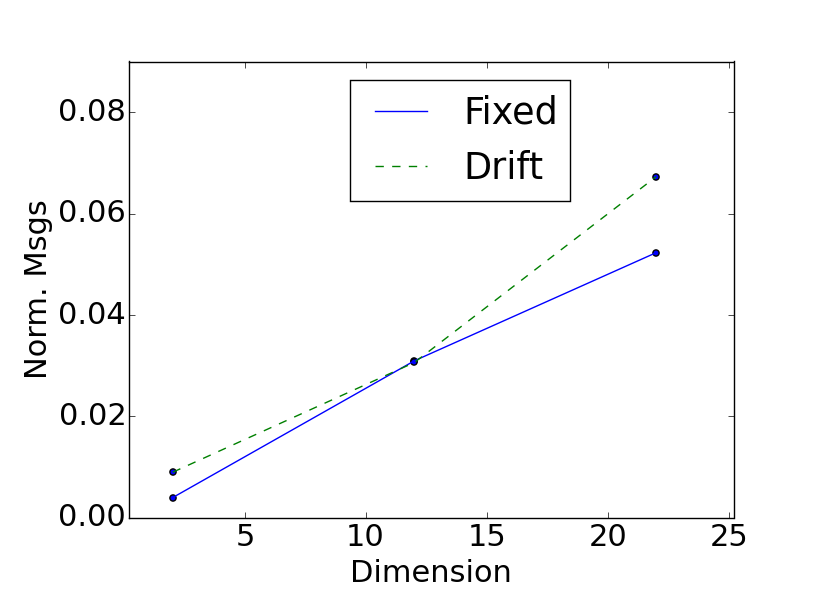
\includegraphics[width=60mm]{CommunicationOfFixedVsDrift/Dimension.png}
	\caption{Communication as a function of input dimension}
	\label{Dimension}
	\end{figure}
\subsubsection{Window Size and Noise}
Figure \ref{WindowSize} shows how communication decreases as a result
of enlarging the window size $W$, which means that $W$ can compensate for other
factors in the system that might increase the communication. One of those is
noise (which is quantified in our context by the standard deviation of the
underlying distribution the data was generated from).
 \begin{figure}[h]
	\centering
	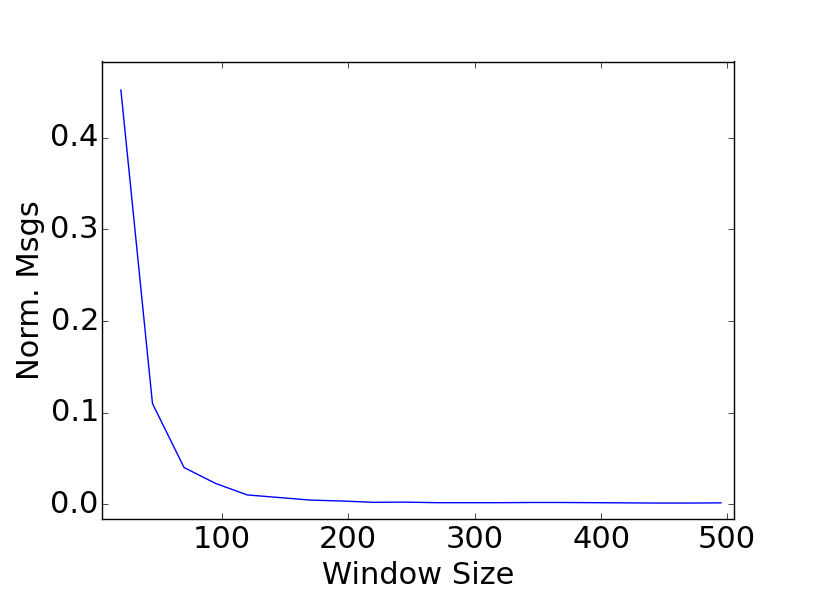
\includegraphics[width=60mm]{CommunicationOfFixedVsDrift/WindowSize.png}
	\caption{Communication as function of window size $W$}
	\label{WindowSize}
	\end{figure}
%\subsubsection{Noise}
Figure \ref{Noise} shows normalized messages obtained at different
noise magnitudes. As expected, the threshold required to preserve a
fixed error increases along with data noise.
\begin{figure}[h]
	\centering
	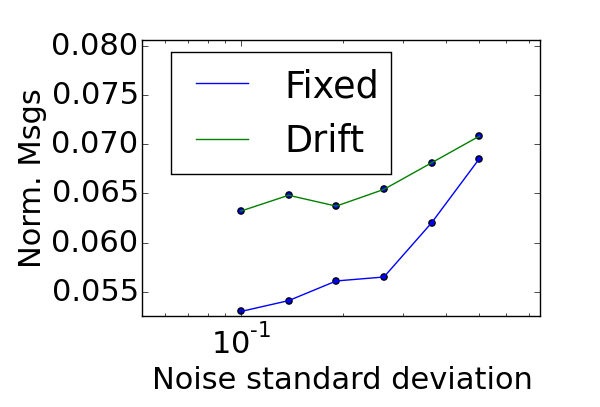
\includegraphics[width=60mm]{CommunicationOfFixedVsDrift/Noise.png}
	\caption{Communication as a function of the standard deviation of the
	distribution according to which the data was generated.}
	\label{Noise}
	\end{figure}

\subsection{Real Data Experiments}
In this section we demonstrate the algorithm with 3 datasets. The first
(newsgroups collection) is relatively small, small enough for using
the deterministic DLDA algorithm and there is no need to use PDLDA.
The second (Power Consumption Monitoring) is a medium size dataset (it
is distributed over 36 nodes) and both DLDA and PDLDA are demonstrated on it. 
The third (Gas Sensor Time Series Monitoring) is big (it is distributed over
100 nodes), so we had to use only PDLDA on in.
\subsubsection{Message Preference Monitoring --- Usenet}
The USENET dataset is described in \cite{usenet}.
This is a text dataset that simulates a stream of messages from three newsgroups
(medicine, space, baseball); the messages are presented sequentially to a user, 
who then labels them as interesting or junk, according to personal interest. 
Attribute values are binary, indicating the presence or absence of the 128
informative words. The drift occurs from an artificial change in the user's
preference (from space to baseball). In Figure \ref{usenet} the behavior of the
DLDA algorithm with $W=450$ is presented. The first 450 rounds over the data are for
initialization and are omitted. During the next 50 rounds the DLDA error 
(the value is calculated on the left side of inequality
\ref{eq:convexBound}) increases due to noise in the data; there is
no concept drift. From round 500 to 600 the DLDA error is stable, 
and again is due only to the noise. In round 600 there is a concept 
drift.
From this point both the DLDA and the true error increase until the 
synchronization in round 698.

\begin{figure}[h]
	\centering
	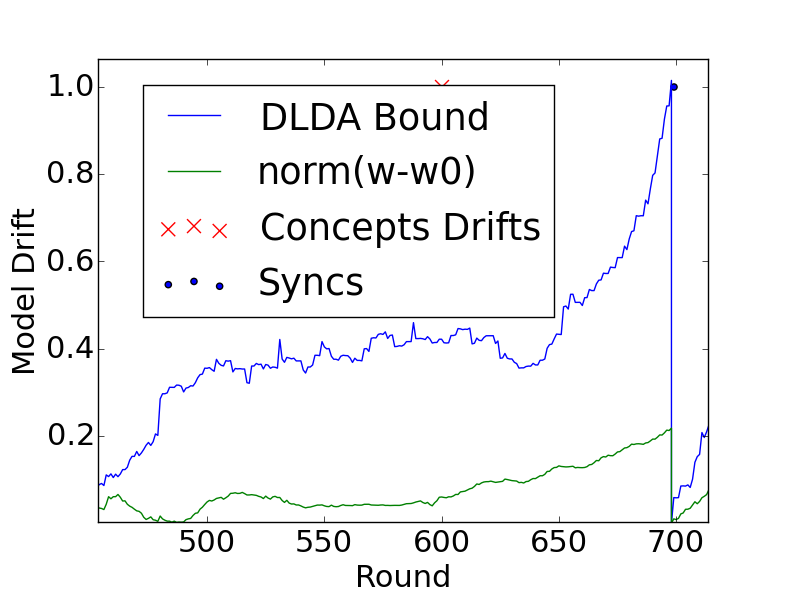
\includegraphics[width=60mm]{Usenet/DriftDetected.png}
	\caption{Comparison between maximal (over nodes) DLDA (blue) 
	error and the true global error (green) for $k=2$, $W=450$. 
	It can be seen that DLDA responds to the concept drift that occurs 
	after 600 rounds (red x) and causes a synchronization in round 698 (blue dot).}
	\label{usenet}
	\end{figure}
	
\subsubsection{Power Consumption Monitoring}
The Power Consumption dataset contains the hourly power supply of an 
Italian electric company as recorded from two sources: power supplied 
by the main grid and power transformed from other grids. 
This stream contains three-year power supply records 
from 1995 to 1998, and our learning task is to predict which hour (1 out of 24 hours) the 
current power supply belongs to. The concept drift in this stream 
is mainly driven by factors such as the season, weather, time of day, 
and the differences between working days and weekend.  
The dataset is described and can be downloaded from \cite{powerSupply}.
We demonstrate the algorithms on the following binary classification problem: 
given a power supply measurement, decide if it is a night or a day. 
This dataset is an example of gradual concept drift (seasons do not
change suddenly).
In Figure \ref{PowerSupplyFigures} DLDA
and PDLDA are demonstrated. For a small number of nodes, $k=4$, and for big
window size, $W=5000$, the communication is reduced to 0.3\%. 
For a more distributed system, k=36, and a smaller window
size, $W=600$, the communication is reduced to 9\%. For PDLDA with
$k=36$ and $W=600$ and a violation threshold (VT) of 50\%, the communication 
is reduced to 2\%.


\begin{figure}[h!]

%\begin{minipage}[c][][t]{.5\textwidth}
  %\vspace*{\fill}
  
  \begin{subfigure}
  \centering
  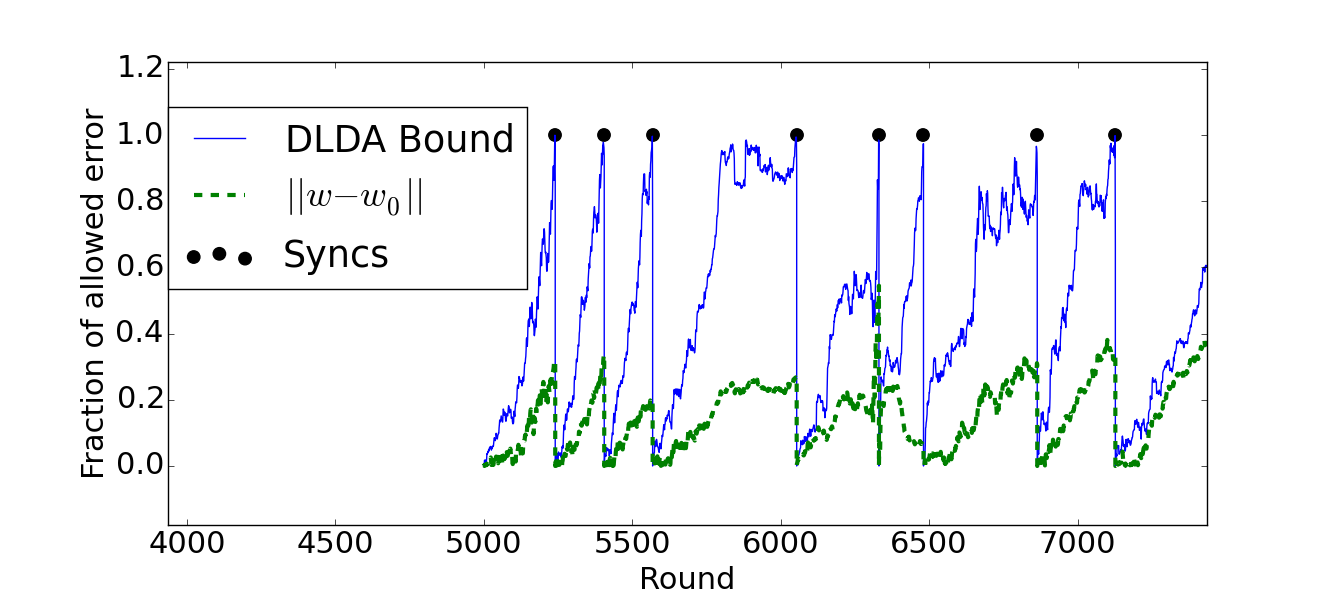
\includegraphics[width=6cm]{PowerSupply/4nodes.png} 
  \label{PowerSupplyFigure1}
  \caption{k=4, W=5000, VT=0}
  \end{subfigure}
  
  \begin{subfigure}
  \centering
  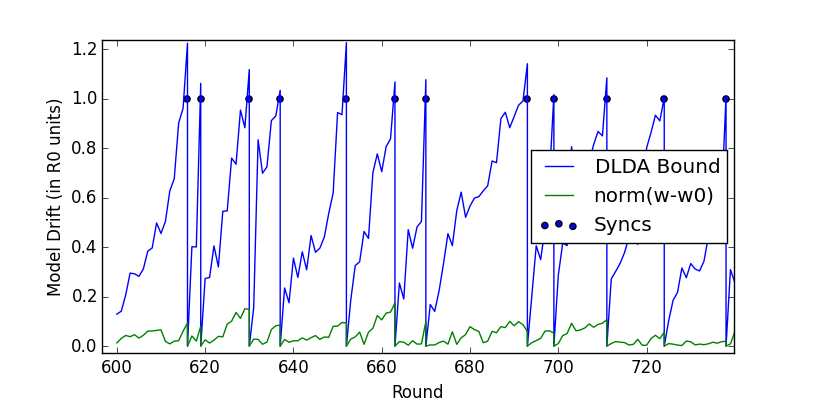
\includegraphics[width=6cm]{PowerSupply/36nodes.png}
  \label{PowerSupplyFigure2}
  \caption{k=36 Nodes, W=600, VT=0}
  \end{subfigure}
  
  \begin{subfigure}  
  \centering
  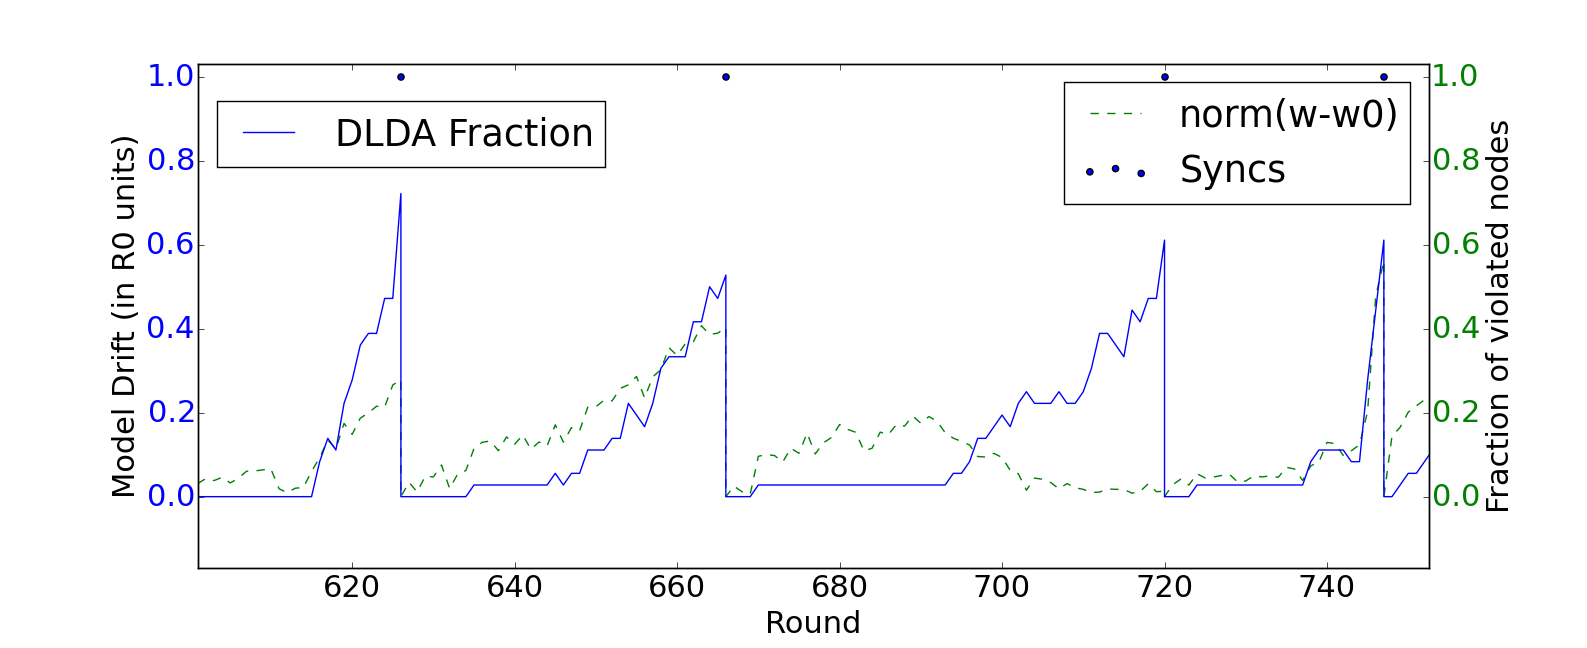
\includegraphics[width=6cm]{PowerSupply/36nodesProb.png}
  \label{PowerSupplyFigure3}
  \caption{k=36 Nodes, W=600, VT=18}
  \end{subfigure}
%\end{minipage}
  \caption{In the first two figures the DLDA algorithm adapts
  to gradual concept drift on the power supply dataset.  
  The maximal error (over the nodes) in the 
  local DLDA bound calculation (blue) is compared to the true
error (the norm of the difference) of all the data aggregated from
all of the nodes (green). In the last figure PDLDA
is demonstrated on the same dataset; the blue curve represents the
fraction of violated nodes.}
\label{PowerSupplyFigures}
\end{figure}

% \begin{figure}[h]  
% 	\vspace{30px}     
%     \fbox{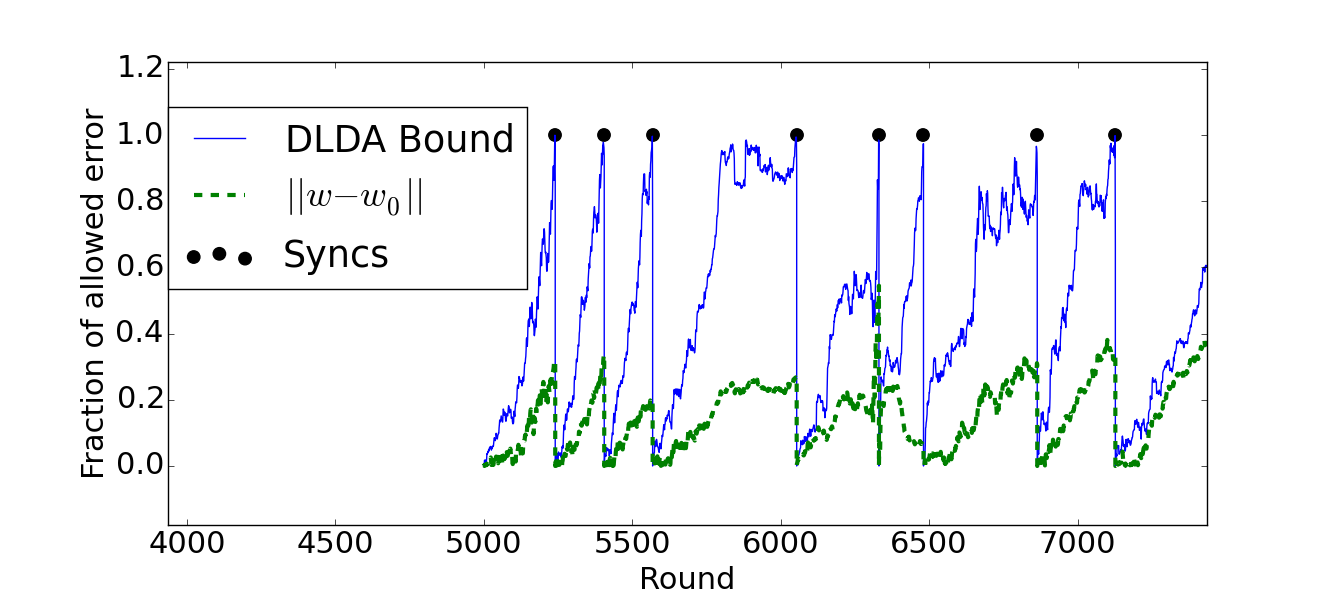
\includegraphics[width=6cm]{PowerSupply/4nodes.png}}   
%     %\vspace{30px}
%     \fbox{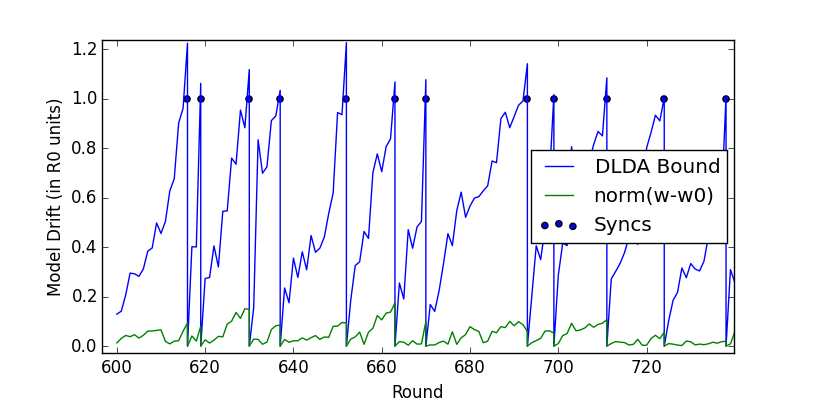
\includegraphics[width=6cm]{PowerSupply/36nodes.png}}
%     %\vspace{30px}
%     \fbox{
%     	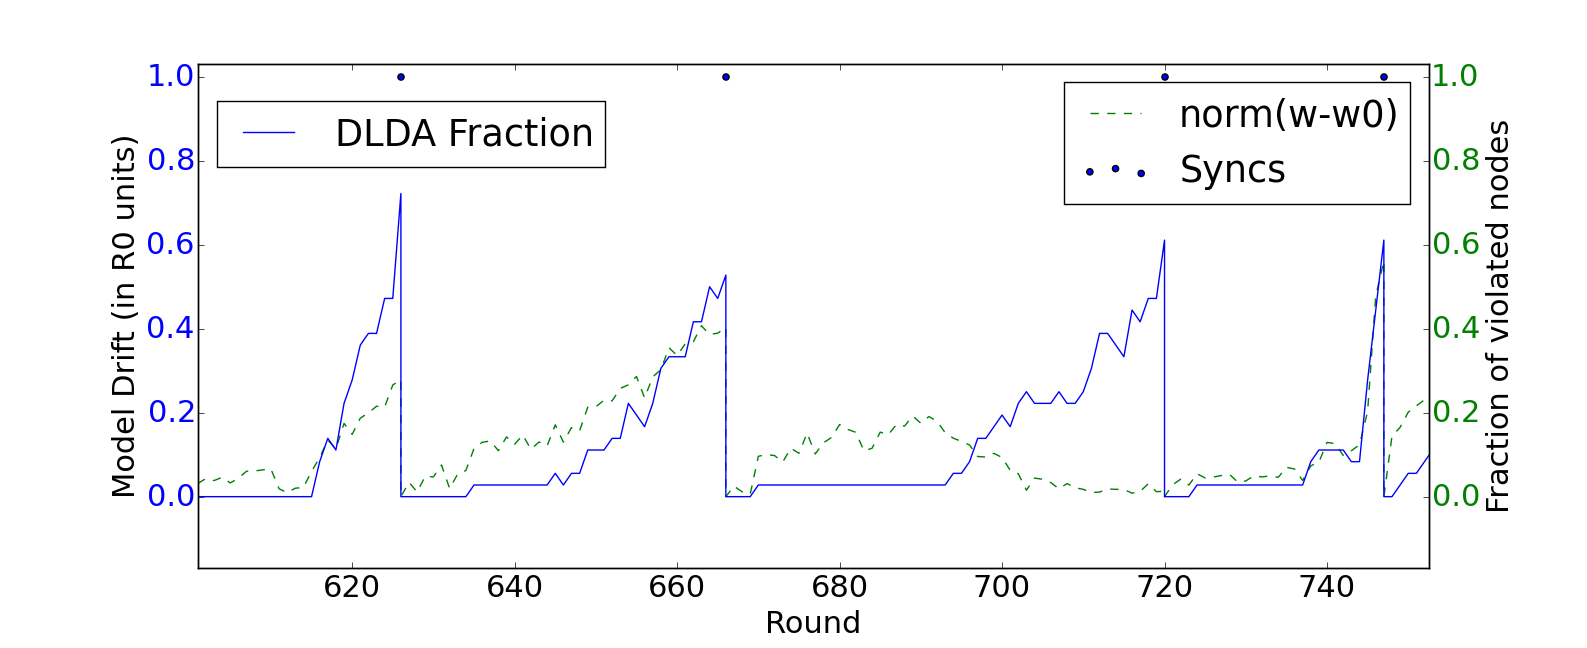
\includegraphics[width=6cm]{PowerSupply/36nodesProb.png}
%     	\caption{k=36 Nodes, W=600, VT=18}
%     }
%     \vspace{10px}
%     \caption{this is the caption}
%     \label{materialflowChart}
% \end{figure}


\subsubsection{Gas Sensor Time Series Monitoring} 

\begin{figure}[h!]
\centering
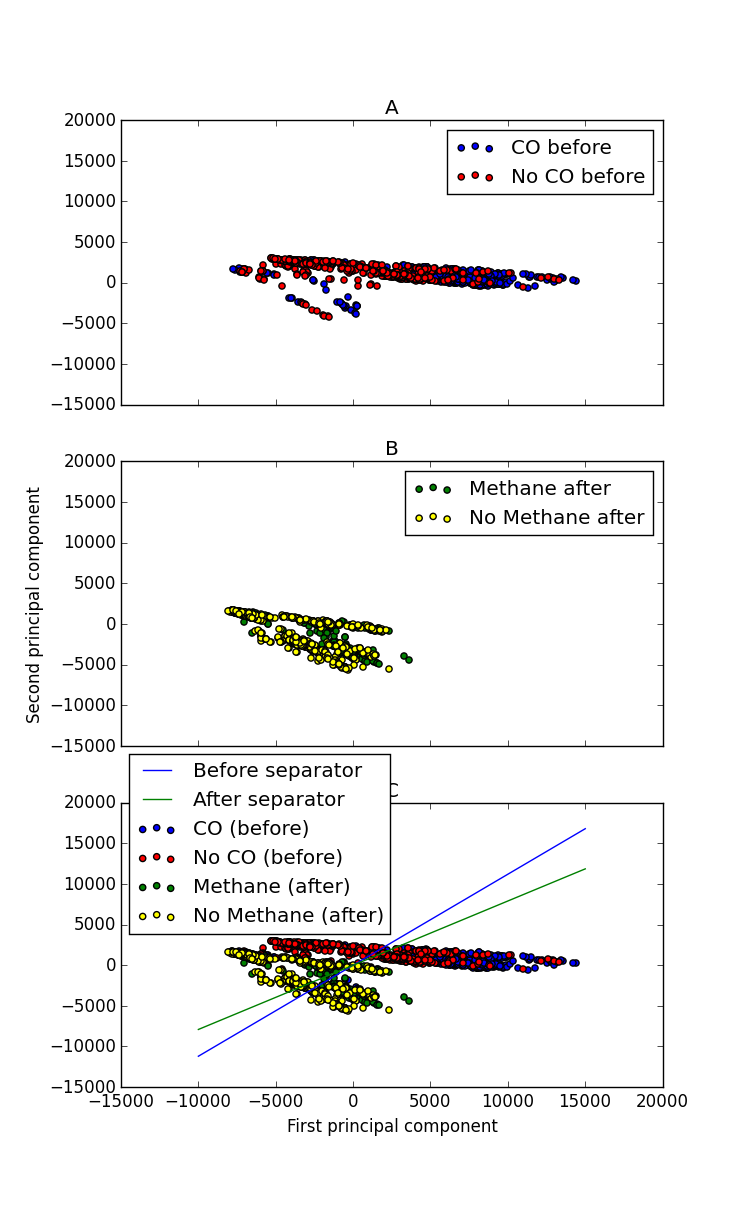
\includegraphics[width=60mm]{BigGas/showData.png}
\caption{Two-dimensional PCA projection of the gas sensor data, 
before concept drift (A), after concept drift (B), 
and the two projections together with their separators (C). 
The plot comes to illustrate the true change in the classifiers angle (as PDLDA
behaviour indicates).}
\label{BigGasShowData}
\end{figure}


\begin{figure*}[ht!]
\centering
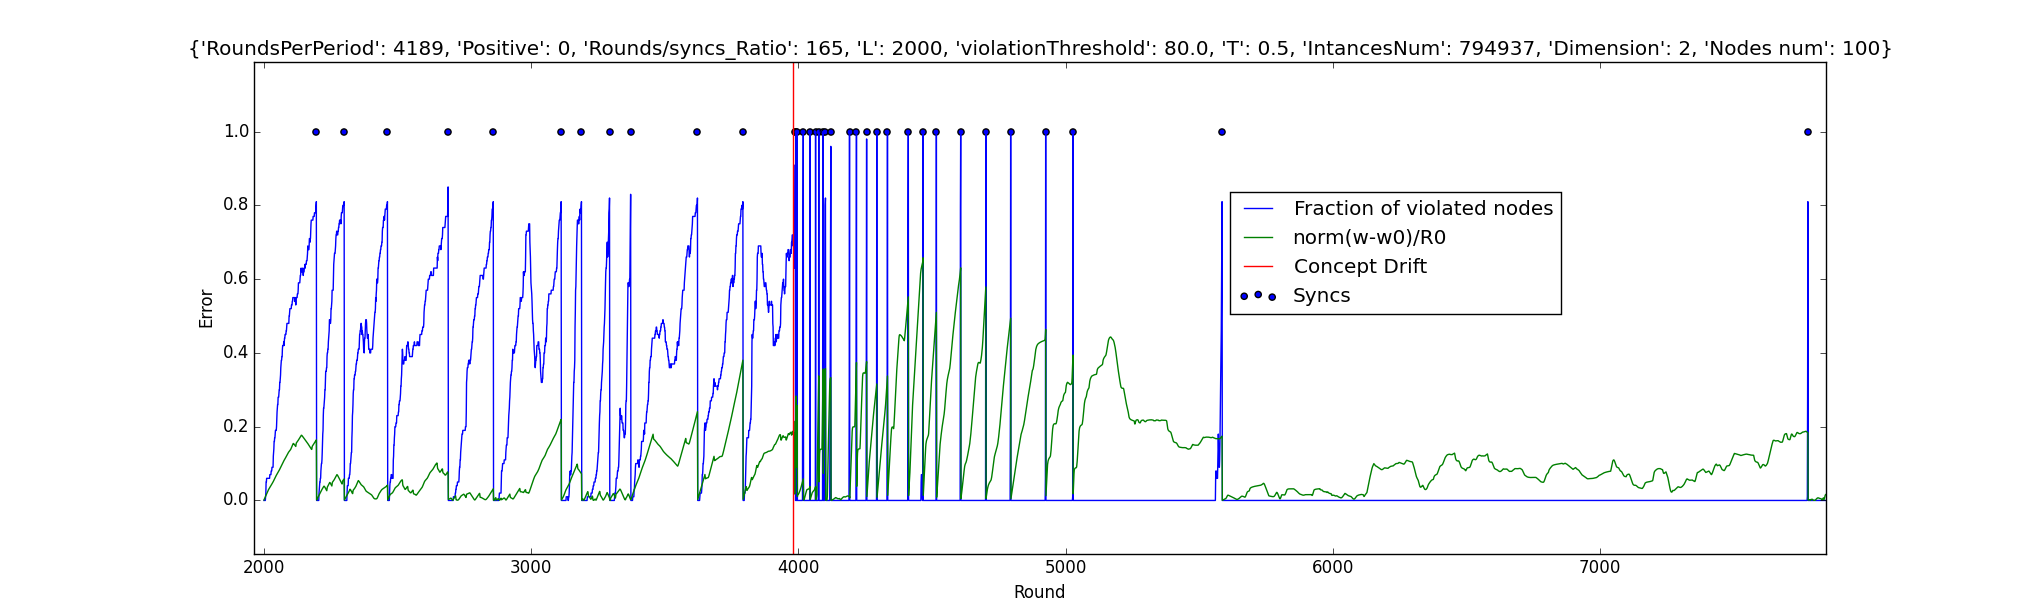
\includegraphics[width=\textwidth]{BigGas/overTime100k.png}
\caption{Demonstration of PDLDA on the Gas Sensor dataset. 
A comparison between the true error (green) to the fraction of the nodes that 
are violated in the current round (blue). 
The experiment is configured for k=100 nodes, and the violation threshold is
VT=80.}
\label{BigGasOverTime}
\end{figure*}
Data in this experiment \cite{bigGas} consists of measurements collected
by an array of 16 chemical sensors in a lab, recording at a sampling
rate of 100Hz for 24 hours, resulting in 8378504 data points for each sensor. 
During the first 12 hours the task is to detect the presence of carbon monoxide
(CO) in a mixture of Gases, and from the 13th hour the task is to detect the presence of methane. 
The change between the first task to the second is the sudden concept drift.
In Fig \ref{BigGasShowData} a PCA projection of the data is shown.
This is a big dataset, and can be massively distributed. 
There are two kinds of drifts in the data: there is a gradual drift that comes from 
the change in temperature in the lab over time, and an
artificial sudden drift that comes from the switch between tasks after 12 hours.
Figure \ref{BigGasOverTime} demonstrate the results of PDLDA.

In Figure \ref{BigGasOverTime} two phenomena can be observed.
First, the two lines are highly correlated --- the fraction of the violated
nodes follows the true error. Second,  before the sudden concept drift 
(marked by the vertical red line), there is a synchronization every 150 rounds, while 
after the concept drift there is a synchronization only every 50 rounds.
The second phenomenon continues over 1000 rounds, where there is a mixture in the 
sliding window between old (before the concept drift) data and new 
(after the concept drift). The existence of the second phenomena shows that
the PDLDA algorithm detects and responds to the sudden concept drift.


\section*{Conclusions}
We introduced the first monitoring algorithm for a linear classifier model.
As long as all of the nodes agree with their local test, the
global model guaranteed to be valid. 
Our algorithm outperforms PER: it maintains a smaller Euclidean distance between 
the last computed model to the current true model with a lower volume of
communication. 
Our empirical study found a linear relationship between the dimension and
communication, something that might also be explained analytically 
in future work. 
We evaluated our algorithm --- DLDA --- and its probabilistic version --- PDLDA --- on 3 real datasets. For a small number of nodes we used 
DLDA with its theoretical guarantee, and for a greater number of nodes we used
PDLDA.
We reduce communication by an order of two magnitudes while maintaining a 
valid model.
 \section*{Acknowledgements}
Thanks to Moshe Gabel for the help in kicking off this research.

%
% The following two commands are all you need in the
% initial runs of your .tex file to
% produce the bibliography for the citations in your paper.
\bibliographystyle{abbrv}
\bibliography{bib}  % sigproc.bib is the name of the Bibliography in this case
% You must have a proper ".bib" file
%  and remember to run:
% latex bibtex latex latex
% to resolve all references
%
% ACM needs 'a single self-contained file'!
%

\appendix
\section{Appendix} \label{AppendixA}
To find a convex subset C satisfying the condition of Eq. \ref{convex},
We first define the operator norm:
\begin{definition}
Let $A$ be a matrix. Its operator norm, or
spectral norm, hereafter just norm, is defined as:
\begin{equation*}
||A|| = \sup_{x \neq 0}\frac{||Ax||}{||x||}.
\end{equation*}
\end{definition}

\begin{lemma} \label{lemma:newman}
If A is square and $||A|| < 1$, then
\begin{equation*}
||(I+A)^{-1}|| < \frac{1}{1-||A||}.
\end{equation*}
\end{lemma}
The proof for this lemma can be found in \cite{gabel2015monitoring}.

\subsection{Convex Bound Proof}
We recall that $\mathcal{C}$ is the convex subset that satisfies 
inequality \ref{convex} and $\mathcal{G}$ is the set of triplets 
$(\Delta_s^i, \delta_p^i, \delta_q^i)$
 that satisfies the inequality \ref{eq:convexBound}.

\begin{lemma}
$\mathcal{G} \subseteq \mathcal{C}$:
\end{lemma}

\begin{proof}
We can write the sphere condition in terms of $B_0, \Delta, u_0$ and $\delta$ using the triangle
inequality:
\begin{equation} \label{in}
\begin{split}
||w-w_0|| & = \ ||(B_0+\Delta)^{-1}(u_0+\delta) - B_0^{-1}u_0|| \\
& < ||(B_0+\Delta)^{-1}\delta|| \\
& \ \ + ||((B_0+\Delta)^{-1} - B_0^{-1})u_0||.
\end{split}
\end{equation}

We split the right side of the last inequality into two parts:
\begin{equation}  \label{e1e2}
\begin{split}
& E_1:= ||(B_0+\Delta)^{-1}\delta|| \\
& E_2:= ||((B_0+\Delta)^{-1} - B_0^{-1})u_0||.
\end{split}
\end{equation}
Under the assumption of $||B_0^{-1}\Delta||\ \leq \ 1$, 
it follows from lemma \ref{lemma:newman}:
\begin{equation} \label{e1e2In}
\begin{split}
& E_1 \leq \frac{||B_0^{-1}\delta||}{1-||B_0^{-1}\Delta||} \\
& E_2 \leq  \frac{|| B_0^{-1}\Delta w_0||}{1-||B_0^{-1}\Delta||}.
\end{split}
\end{equation}
From the Cauchy-Schwarz inequality we get:
\begin{equation} \label{CS}
||B_0^{-1}\Delta w_0|| \ \leq \ ||B_0^{-1}\Delta||||w_0||.
\end{equation}
Substituting Eq. \ref{e1e2}, \ref{e1e2In} and \ref{CS} in Eq. \ref{in}, we
get:
\begin{equation}
\begin{split}
|| w-w_0 \parallel & \leq \ E_1+E_2 \\
& \leq \frac{||B_0^{-1}\delta|| + ||B_0^{-1}\Delta||||w_0||}{1 -||B_0^{-1}\Delta||} \\
& \leq R_0.
\end{split}
\end{equation}
After rearranging the terms, we get
\begin{equation} \label{lostDenom}
||B_0^{-1}\delta|| + ||B_0^{-1}\Delta||||w_0||.
\leq R_0(1 -||B_0^{-1}\Delta||)
\end{equation}
From the triangle inequality we can rewrite:
\begin{equation} \label{linQuad}
||B_0^{-1}\Delta|| \leq ||B_0^{-1}L||+||B_0^{-1}M||.
\end{equation}
And finally, combining inequalities \ref{lostDenom} and \ref{linQuad},
we get the following bound:
\begin{alignat*}{2} \label{convexBound}
&||B_0^{-1}\delta|| &+ (||w_0||+R_0)(||B_0^{-1}L||+||B_0^{-1}M||) && \\ 
& \leq R_0. &&
\end{alignat*}
\end{proof}

\begin{lemma} \label{delta}
$||B_0^{-1}\delta||$ is convex in $\delta$.
\end{lemma}
\begin{proof}
Multiplication by $B_0^{-1}$ is a linear operation and norm is convex
operation. Therefore $||B_0^{-1}\delta||$ is convex in $\delta$.
\end{proof}

We recall that:
\begin{equation*} 
L:= \Delta_S - p_0\delta_p^T - \delta_pp_0^T - q_0\delta_q^T - \delta_qq_0^T.
\end{equation*}
\begin{lemma} \label{L}
$||B_0^{-1}L||$ is convex in $\Delta_s, \delta_p$
and $\delta_q$.
\end{lemma}
\begin{proof}
$L$ is linear in the variables and therefore convex in these variables.

\end{proof}

We recall that:
\begin{equation*} 
M:= - \delta_p\delta_p^T - \delta_q\delta_q^T.
\end{equation*}

\begin{lemma} \label{M}
$||B_0^{-1}M||$ is convex in $\delta_p$
and $\delta_q$.
\end{lemma}
\begin{proof}
From the definition of operator norm, we can rewrite the function as:
\begin{alignat*} {2}
||M|| & = && ||B_0^{-1}(\max_{||u||=1}{\{u^T \delta_p\delta_p^T u\}} +
\max_{||u||=1}{\{u^T \delta_q\delta_q^T u\}})||\\
& = && ||B_0^{-1}(\max_{||u||=1}{\{||u^T \delta_p||^2\}} +
\max_{||u||=1}{\{||u^T \delta_q||^2\}})||.
\end{alignat*}
We observe that max over a finite number of convex functions is also a convex
function, multiplication by a matrix and the norm keeps it convex.
This concludes our proof.
\end{proof}

\begin{corollary}
From lemmas \ref{delta}, \ref{L} and \ref{M} we can conclude that $\mathcal{G}$
is convex.
\end{corollary}
\end{document}
